This chapter presents the results of the conducted experiments. First, an overview of the results achieved with the entire system is given. Subsequently, individual components of the system are examined in more detail.
The code and documentation are made publicly available. Further information can be found in \chref{online_sources}.

\section{Entire System}
%
\begin{figure}[h]
    \centering
    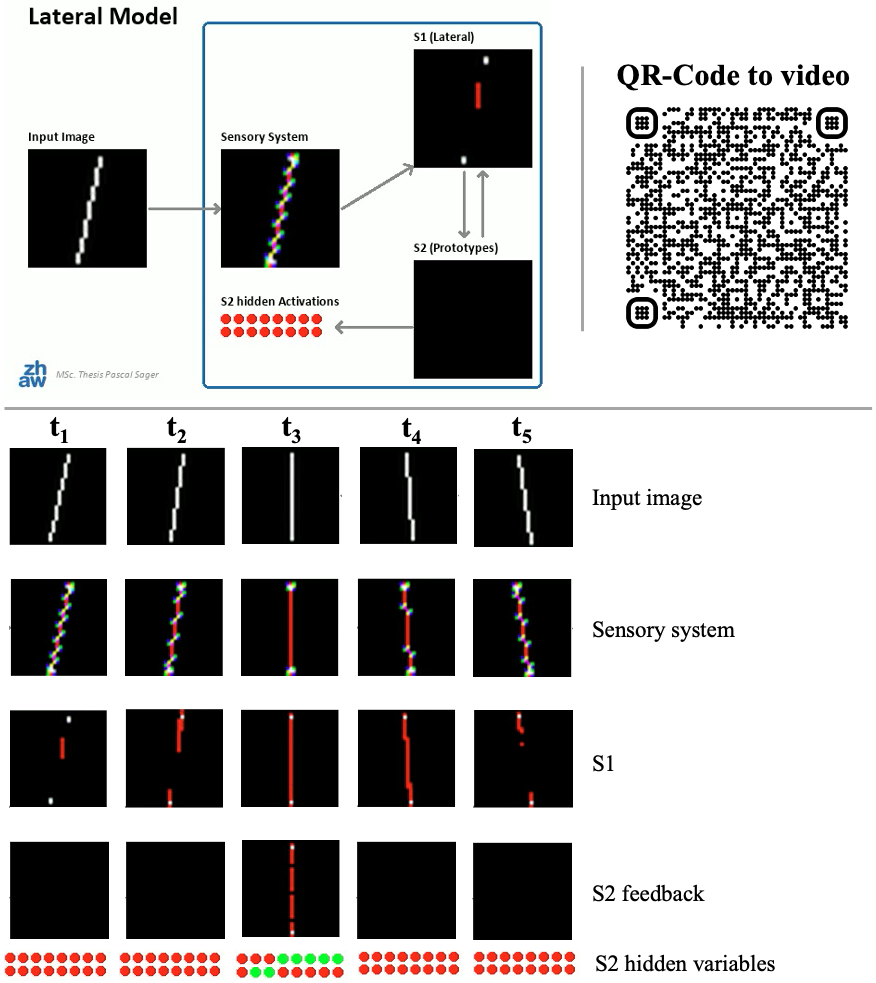
\includegraphics[width=0.99\textwidth]{r1_overview}
    \caption[Frames of a video visualising the model's activations]{Frames of a video visualising the model's activations. At the top of the image, an actual video frame and a QR code to the video are shown. At the bottom of the image, the changing network activations over time are visualised.}
    \figlbl{r1_overview}
\end{figure}
%
An overview of the entire system is provided in \figref{r1_overview}.
This figure is derived from a video available at \url{https://sagerpascal.github.io/lateral-connections/results/final_results.html#video-visualisations} or with the QR code on the top right of the figure.
For a detailed explanation of the components shown in the video, please refer to \secref{result_video}.
The figure shows the network's activations for a line rotated counterclockwise around its centre.

The network has only been trained on vertical, horizontal, and diagonal lines.
Therefore, many lines fed into the network in this video represent unknown objects.
However, \emph{S1} still detect some learned patterns, such as multiple pixels aligned vertically, horizontally, or diagonally.
Therefore, it can provide lateral support between local pixel groups representing such a pattern.
The closer the input becomes to a learned pattern, the bigger the lateral support.
At time $t_3$, the input corresponds to a vertical line as observed during training.
In that case, all pixels receive enough lateral support to remain active.

For the conducted experiments, \emph{S2} does not map the net fragments to a reference frame but acts as a memory of learned objects.
It is needed to provide feedback and is considered a mockup that has to be replaced in future work by a network implementing projection fibres.
As long as the net fragments represent an unknown pattern, no latent cells in \emph{S2} are activated and no feedback to \emph{S1} is provided.
However, when the net fragments in \emph{S1} correspond to a learned pattern, \emph{S2} provides feedback and further increases certainty in \emph{S1}.

Overall, the network's behaviour is as expected: \emph{S1} builds net fragments based on well-known patterns.
These patterns provide support to each other to remain active.
\emph{S2} only responds to patterns stored in its memory, therefore only providing support to \emph{S1} for previously seen patterns.

Furthermore, all samples seen during training have automatically been saved in \emph{S2}.
The system is able to produce net fragments that roughly reassemble the input from the sensory system.
However, compared to the sensory system, the net fragments are more robust as shown in the following sections.





















% TODO: From here on correct text:




\subsection{Adding Noise}
%
\begin{figure}[h]
    \centering
    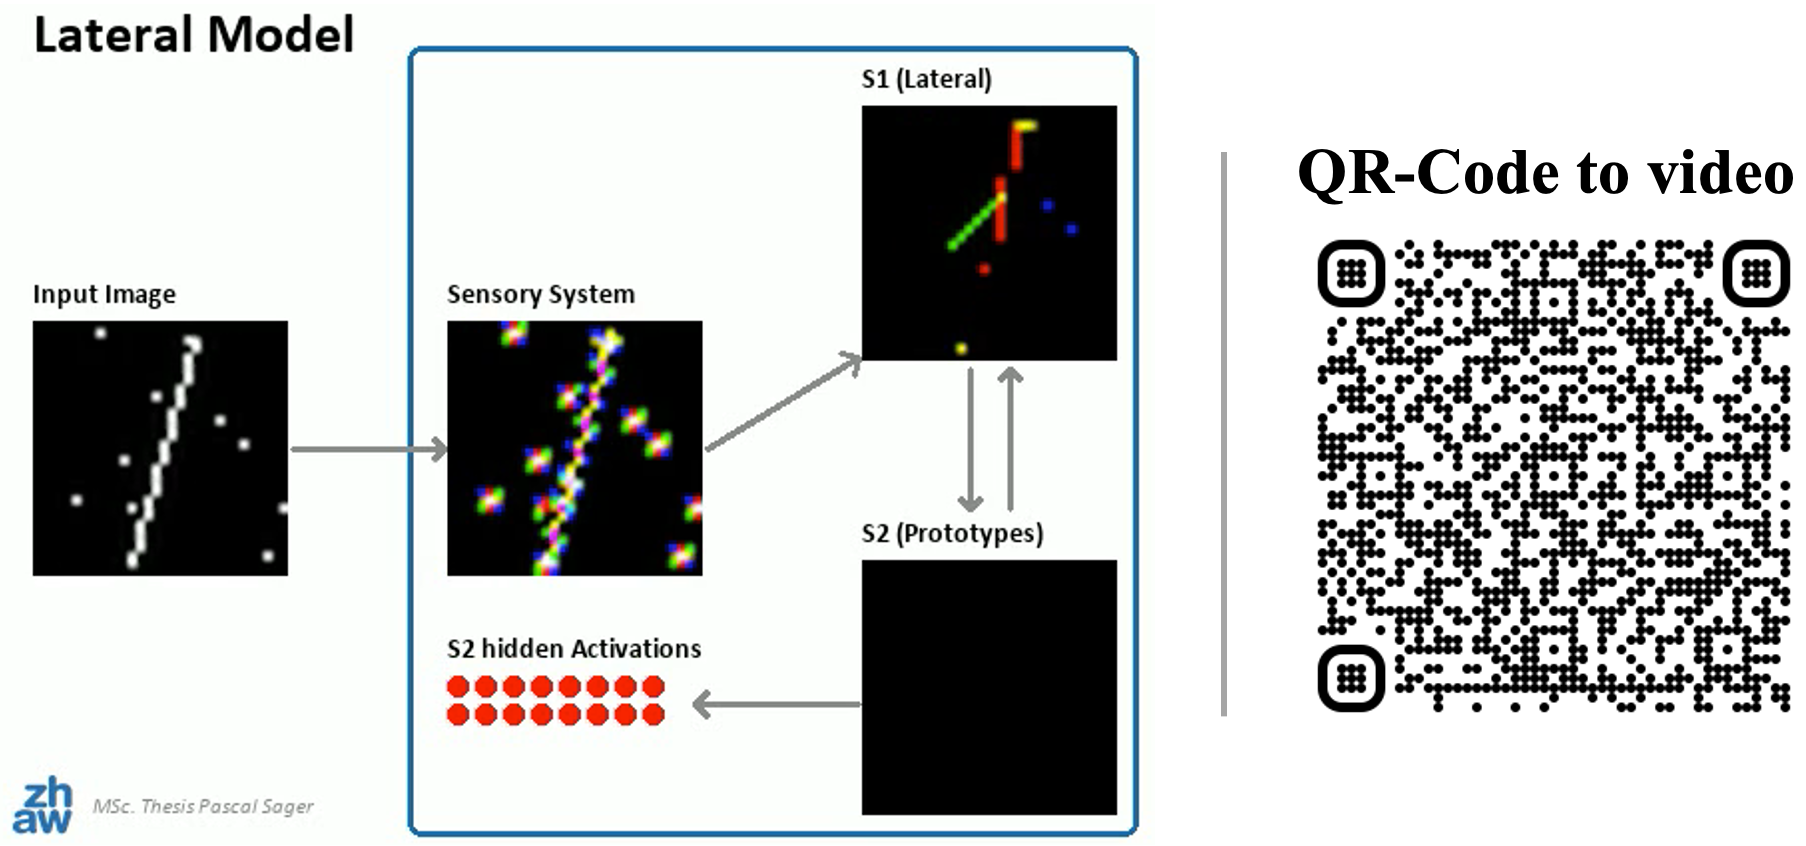
\includegraphics[width=0.99\textwidth]{r2_overview}
    \caption[Video visualising the network's behaviour with noise in input]{A frame of a video visualising the network's behaviour if noise is added to the data. The QR code on the right links to the corresponding video.}
    \figlbl{r2_overview}
\end{figure}
%
\figref{r2_overview} refers to a video demonstrating the network's behaviour is noise is added to the input data.
Noise is added by flipping a pixel from $0$ to $1$ or vice versa in the input data with a probability of $0.005$.
On average, this leads to $5.12$ pixels changing their activity.

To measure how well the model can deal with noise, the same input is fed twice into the model, once with noise and once without.
The sensory system's activations of these two image versions are compared, and the percentage of feature cells that are triggered by noise and subsequently turned off is measured.
The system is able to remove about $71.2\%$ of the noise.
However, this is mainly because a single noise pixel triggers about $3$ cells in each feature channel, leading to $12$ active cells, from which only the $4$ feature cells at the centre remain active after processing. Thus, the noise is not actually removed but only reduced.

\begin{figure}[h]
    \centering
    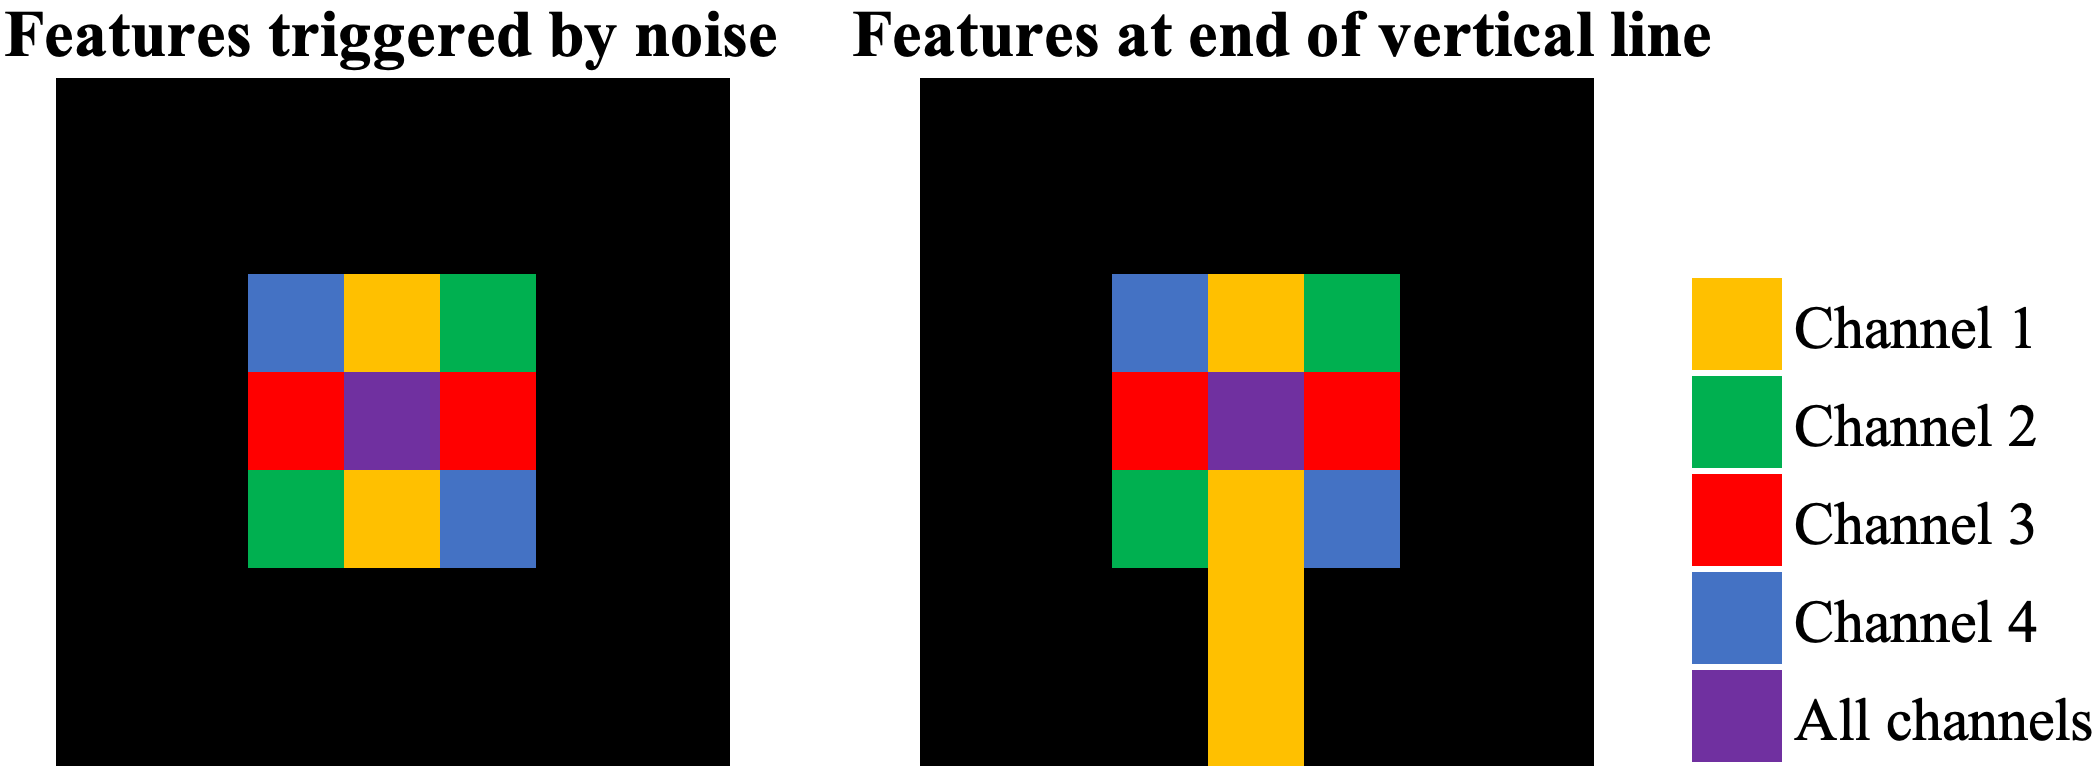
\includegraphics[width=0.49\textwidth]{features_noise_data}
    \caption[Features triggered by noise]{.}
    \figlbl{features_noise_data}
\end{figure}
%
Only in $17.8\%$ of the cases is noise in the input completely removed. There exist several reasons why noise is not well removed: First, noise can be located close to the line or other noise and thus receive support from other cells. Second, noise in the input triggers all feature channels and is similar to activations that can be found at line ends as visualised in \figref{features_noise_data}.
Thus, these cells should support each other and can not be adequately filtered by the system.

Although the noise cannot be completely filtered out, the net fragments are still mapped to the correct prototype in \emph{S2}. Thus, the input is correctly interpreted by the system despite the noise.

\subsubsection{Noise per Channel}
%
\begin{figure}[h]
    \centering
    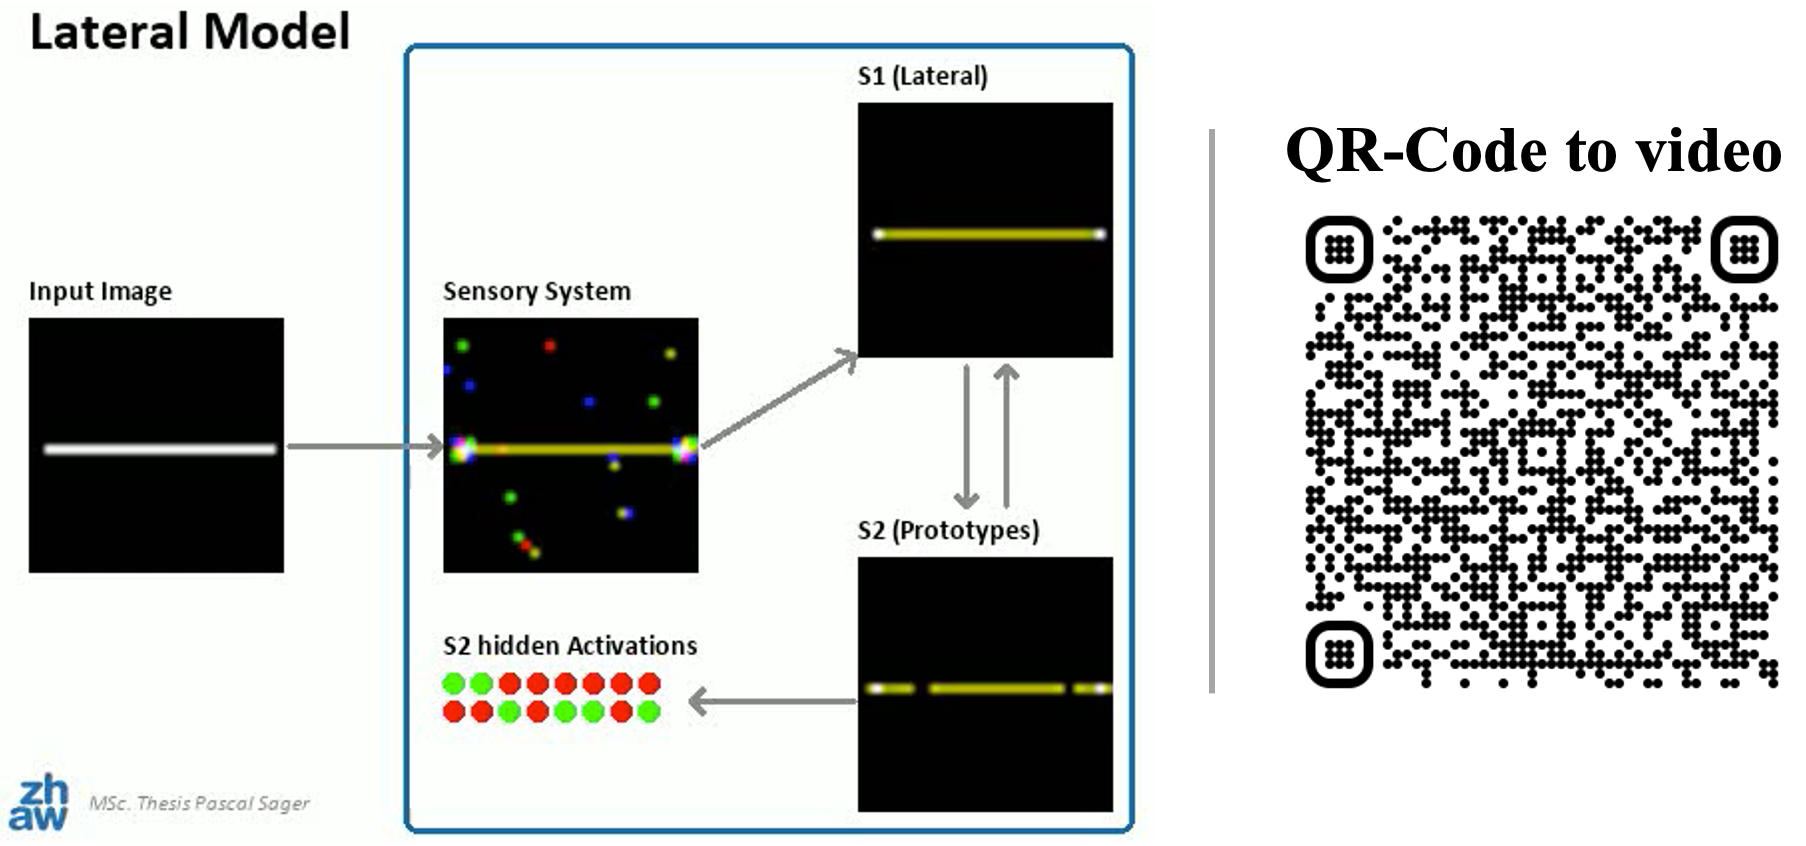
\includegraphics[width=0.99\textwidth]{r3_overview}
    \caption[Video visualising the network's behaviour with noise in the feature channels]{A frame of a video visualising the network's behaviour if noise is added to the feature channels. The QR code on the right links to the corresponding video.}
    \figlbl{r3_overview}
\end{figure}
%
It is also investigated whether noise can be filtered when no correlation exists between the locations in the feature channels.
Therefore, noise is not added to the input data but directly to the feature channels of the sensory systems' output.
It is presumed that this better corresponds to a real-world scenario where such a network most likely has, by factors, more input channels, and it is highly unlikely that noise is highly similar to a learned pattern that seems valid.

\figref{r3_overview} refers to a video demonstrating the networks' behaviour when noise is added to each feature cell with a probability of $0.005$.
In this case, about $91.7\%$ of the noise is removed, demonstrating the network's high robustness.


\subsection{Interrupted Line}
%
\begin{figure}[h]
    \centering
    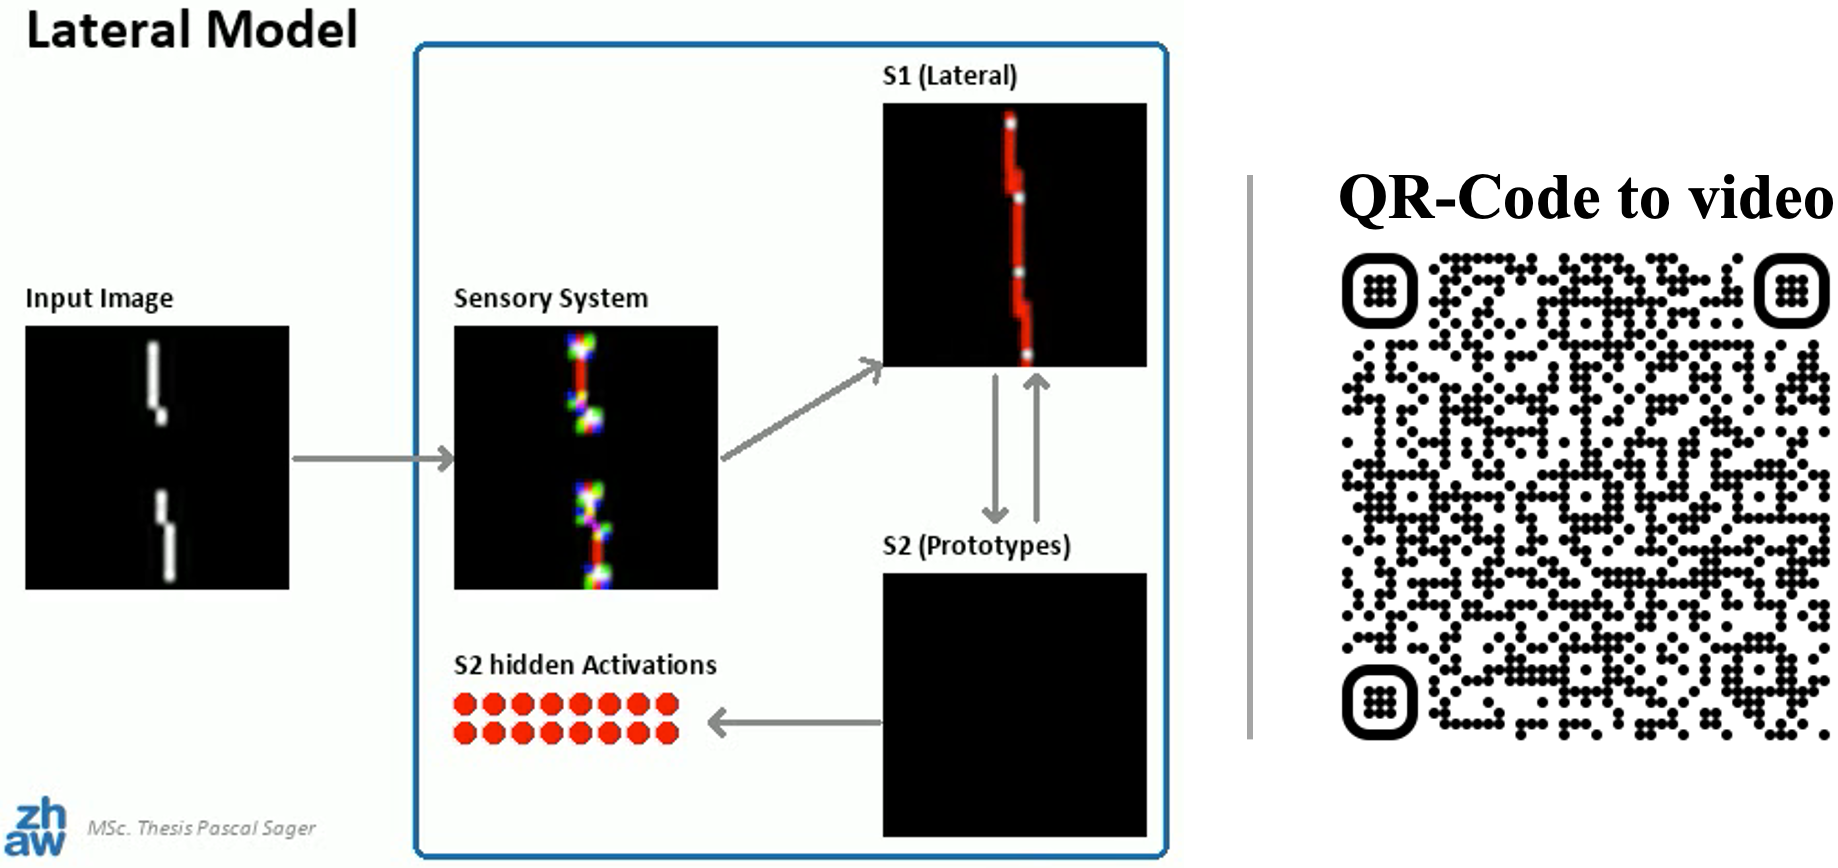
\includegraphics[width=0.99\textwidth]{r4_overview}
    \caption[Video visualising the network's behaviour for discontinuous lines]{A frame of a video visualising the network's behaviour for discontinuous lines. The QR code on the right links to the corresponding video.}
    \figlbl{r4_overview}
\end{figure}
%
Lateral connections can not only reduce noise but also recreate overlaid objects.
This is demonstrated by analysing the network's behaviour if a discontinuous line is fed into the network.
\figref{r4_overview} contains a QR code linking to a video demonstrating that the model is able to recreate lines that are interrupted by up to $8$ pixels.
In the conducted experiments, the centre of the line is detected, and a different number of pixels are turned off.
It is found that the model can always reconstruct the training input if up to $6$ pixels are missing.
It also works in many cases if $8$ pixels are turned off but not if more than $8$ pixels are missing.
The number of occluded pixels that can be reconstructed depends on the reach $n_l$ of the lateral connections.
As expected, increasing $n_l$ allows reconstructing discontinuous lines with more missing pixels.
However, $n_l$ should not be too large so that \emph{S1} build net fragments based on local features (c.f. \secref{TODO}).

In the conducted experiments, the lateral reach is set to $n_l=11$.
Since up to $8$ pixels can be reconstructed, it is argued that restoring object works well.


\section{Model Weights}
%
\begin{figure}[h]
    \centering
    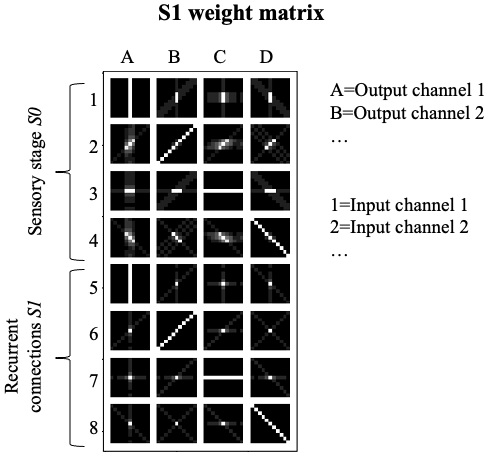
\includegraphics[width=0.79\textwidth]{S1_weight_matrix}
    \caption[Weight matrix of \emph{S1} after training]{The weight matrix of \emph{S1} after training.}
    \figlbl{S1_weight_matrix}
\end{figure}
%
\figref{S1_weight_matrix} visualises the weight matrix of \emph{S1}, representing the learned lateral connections.
\emph{S1} has four output channels, and the kernels contributing to each output channel are depicted in columns labelled from $A$ to $D$.
The input of \emph{S1} consists of four input channels from the sensory stage (rows labelled as $1$-$4$) and four channels from recurrent connections (labelled as $5$-$8$).
Each output channel specialises in a different type of line: Output channel $A$ focuses on vertical lines, channel $B$ on diagonal lines with a positive slope, channel $C$ on horizontal lines, and channel $D$ on diagonal lines with a negative slope.

In the following, output channel $A$ focusing on horizontal lines is discussed.
However, the four output channels are highly similar, except the filters are rotated by $45°$.
Consequently, the insights gained from the analysis of channel $A$ can also be transferred to all other channels.

\begin{figure}[h]
    \centering
    \includegraphics[width=0.99\textwidth]{S1_weight_analysis}
    \caption[Analysis of weight matrix]{An overview of the data processed by the weight matrix of \emph{S1}.}
    \figlbl{S1_weight_analysis}
\end{figure}
%
\figref{S1_weight_analysis} shows the features that are processed when a horizontal line is fed into the system.
First, the sensory system extracts four features (visualised in the grey box named ``output sensory system'').
Channel $1$ contains ``vertical-line features'', spanning the entire vertical length of the image. 
The channels $2$-$4$ contain features of diagonal and horizontal lines. However, the sensory system recognises these features only at the ends of the lines.
Thus, at the ends of the vertical line, about three neurons respond for each channel $2$-$4$ to represent these features.
As expected, these features have been incorporated into the weight matrix accordingly (see $A1$-$A4$).

Based on these features, output channel $A$ generates a response roughly corresponding to the vertical line originally fed into the system.
Thus, channel $A$ fulfils its purpose and represents vertical lines.
Besides channel $A$, also the channels $B$-$D$ become active.
However, these channels specialise in different lines and are only slightly activated.
In fact, these channels activate exactly one pixel at the line ends where the sensory system produces a very high activity across all channels.
Thus, many cells are active at the line end supporting each other.
This activity is sufficient to activate one cell in the output channels $B$-$D$.

The output of \emph{S1} is reused as input signal in the next timestep $t+1$.
This is implemented as a recurrent connection between the output channels $A$-$D$ and the input channels $5$-$8$.
As expected, the filters processing the recurrent input for output channel $A$ specialise in the activity that is produced for vertical lines:
When a vertical line is processed, the output channel $A$ produces a vertical line and the channels $B$-$D$ a single-pixel activity corresponding to the filters $A5$-$A8$.


\subsection{Weight Normalisation}
As described in \secref{TODO}, the weight is normalised in the range $0, ..., 1$.
This ensures that the lateral support is not dominated by a single cell.
Without normalising the weights, the lateral support grows to infinite if trained long enough.
In the human brain, however, such dominant cells do not exist, and neighbouring cells are similarly important in providing support \sidecite{TODO}.


\begin{figure}[h]
    \centering
    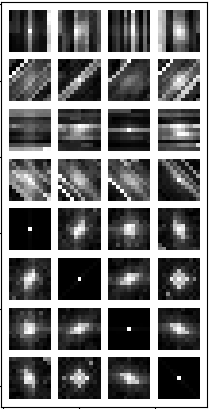
\includegraphics[width=0.49\textwidth]{weights_no_norm}
    \caption[Weights after training without normalisation]{Weight matrix of \emph{S1} after training without weight normalisation.}
    \figlbl{weights_no_norm}
\end{figure}
%
After $10$ epochs, some lateral connections reach a weight above $74$ and dominate the decision process if a neighbouring cell should remain active.
This, in turn, leads to undesired activations and weight updates. 
\figref{weights_no_norm} shows the weight matrix after training if no weight normalisation is used.
No clear structure is visible, and support is provided rather randomly within the network.
Thus, normalisation is not only biologically more plausible but also a necessity to obtain meaningful lateral weights.


\section{Support Goodness}
%
\begin{figure}[h]
    \centering
    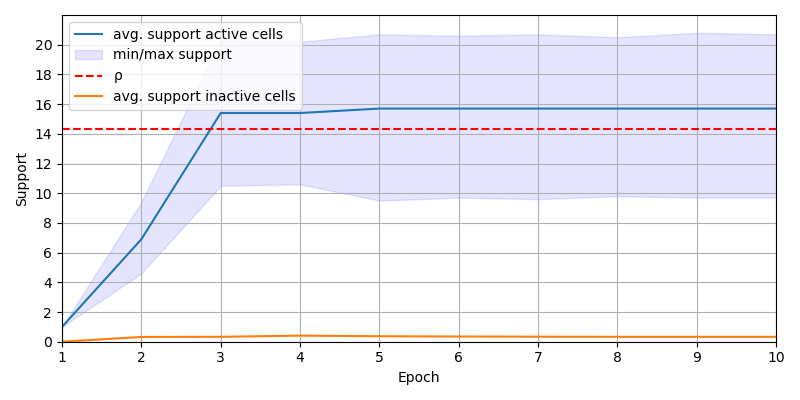
\includegraphics[width=0.99\textwidth]{support_strength}
    \caption[Average lateral support]{The average lateral support received by active and inactive cells during training. The y-axis shows the support and the x-axis the training epoch. The blue line is the average support an active cell receives during training, the light blue interval is the min./max. support active cells receive, and the orange line is the average support inactive cells receive. The dotted red line is the inhibition limit $\rho$ marking the point where the support is reduced.}
    \figlbl{support_strength}
\end{figure}
%
\figref{support_strength} presents the support strength received by active and inactive cells during training before the activation strength is normalised and translated into an activation probability.
Before training, only self-support exists, i.e. the received support for active cells is $1$.
After training for $3$ epochs, the average support active cells receive increases to $15.7$.
At this point in training, most lateral connections have converged to a synaptic weight strength of $1$.
Thus, a single cell is supported by approximately $15$ neighbouring cells on average.
Inactive cells, on the other hand, do not receive considerably more support after training. Inactive cells receive on average a lateral support of $0.3$, significantly less than active cells.

The support active cells receive could increase further but is limited by the inhibitory strength $\rho = 1.3\cdot n_l = 14.3$.
When a cell exceeds this threshold $\rho$, its activation probability is linearly reduced, and cells might become inactive.
Experiments show that cells can receive lateral support strengths up to $20$ when no inhibitory signals are present in the network (c.f. \secref{TODO}).
However, such strong support leads to undesired effects as discussed in \secref{TODO}.
When using a threshold, the model tends to find a trade-off that only slightly surpasses this inhibition limit, thereby maximising the lateral support each cell receives while still ensuring that each cell has a high activation probability.

The results depicted in \figref{support_strength} demonstrate that \emph{S1} builds net fragments as expected. The gap between the support strength of active and inactive cells becomes bigger during training, ensuring that only cells representing known patterns remain active.









\section{S2 Feedback}

\section{Inhibition}

\section{Initialisation}

\section{Winner-Take-All}

\section{Negative Hebbian Learning}


